
Несмотря на значительные усилия сотрудников ГИБДД по разработке и реализации мероприятий, способствующих обеспечению безопасности дорожного движения \cite{KrudorCam}, статистика дорожно-транспортных происшествий (ДТП) как в Российской Федерации (РФ) в целом, так и в отдельных регионах, говорит о большом количестве происшествий с тяжкими телесными повреждениями и летальным исходом. Например рост ДПТ на железнодорожных переездах по данным Краевого государственного казённого учреждения <<Управление автомобильных дорог по Красноярскому краю>> (КГКУ <<КРУДОР>>) с 2016~г. по 2017~г. составил 38~\% с пострадавшими 79~\% \cite{KrudorDTP}. 

Одним из факторов, способствующих возникновению опасности для движения транспортных средств и пешеходов, а также созданию аварийных ситуаций на дорогах является активное использование мобильных телефонов водителями во время движения \cite{Pegin2009}.

Правилами дорожного движения Российской Федерации (абз. 6, п. 2.7) водителю запрещено пользоваться во время движения телефоном, не оборудованным техническим устройством, позволяющим вести переговоры без использования рук \cite{PDD}, а Кодексом РФ об административных правонарушениях (ст. 12.36.1) предусмотрена административная ответственность за нарушение этого правила с санкцией в виде денежного штрафа, размером 1500 руб. \cite{KoAP}. 

Однако, не взирая ни на законодательные акты, ни на кричащие цифры статистики ДТП, водители продолжают активно пользоваться мобильными
телефонами, осуществляя управление транспортным средством одной рукой, не прерывая разговоров даже при выполнении таких сложных маневров, как поворот налево, на перекрестках с различным количеством полос движения, разворот на перекрестке, обгон и др. Безусловно, такими действиями создается реальная угроза безопасности всех участников дорожного движения.

Идея данной работы "--- принудительное ограничение возможности телефонных разговоров водителей, управляющих транспортным средством при движении на особо опасных участках автомобильных дорог. Такого эффекта можно достичь двумя способами:
\begin{itemize}
	\item использованием генераторов помех (ГП, анг. jammer), устанавливаемых в непосредственной близости от опасных участков;
	\item подменой базовой станции (БС) оператора сотовой связи в районах опасных участков автодорог. 
\end{itemize}

Однако, использование ГП на перекрестках и опасных участках не целесообразно из-за отсутствия возможности вызвать оперативные службы спасения. Однако, такие устройства довольно популярны и могут, например, применяться на автозаправочных станциях (АЗС), так как на них имеется персонал, следящий за безопасностью. %Примерами таких устройств являются: аллигатор Super 100 "--- это стационарное устройство, питающееся от сети 220 В, 60 Вт, работающее в трех частотных диапазонах: 800, 1800 МГц и 3G с радиусом покрытия до 100 метров. Средняя рыночная стоимость 17 000 руб.; Intercept 1321 "--- это jammer предназначенный для установки на автозаправочных станциях. Эффективно подавляет сотовую сеть в радиусе до 100 метров. Средняя рыночная цена 80~000 руб.

% \begin{table}[ht]
% 	\caption{Технические характеристики}
% 	\label{tbl:TTX}
% 	\centering
% 	\footnotesize
% 	\begin{tabularx}{\textwidth}{|r|X|}
% 		\hline
% 		\textbf{Наименование характеристики} & \textbf{Значение характеристики}                                   \\ \hline
% 		\hline
% 		Производитель                        & Intercept                                                          \\ \hline
% 		Категория                            & jammers                                                            \\ \hline
% 		Стандарт                             & GSM/900/1800/850/1900 - CDMA/450/800/1900                          \\ \hline
% 		Частоты, МГц                         & 425-475, 851/869-894, 925/935-960, 1805-1880, 1930-1990, 2110-2170 \\ \hline
% 		На выходе, Вт                        & 45                                                                 \\ \hline
% 		Питание, В                           & 110/220                                                            \\ \hline
% 		Радиус действия, м                   & 100                                                                \\ \hline
% 		Аккумулятор                          & Опционально                                                        \\ \hline
% 		Антенна                              & Всенаправленная 3-4 dBi, Направленная до 7-8 dBi (опционально)     \\ \hline
% 		Кол-во каналов                       & 4                                                                  \\ \hline
% 		Комплект поставки                    & jammer, Антенны, блок питания                                      \\ \hline
% 		Размеры (ВxШxД), см                  & 36.5~x~25~x~48                                                     \\ \hline
% 		Вес, кг                              & 30                                                                 \\ \hline
% 	\end{tabularx}
% \end{table}

Для ограничения возможностей сотовых телефон предлагается использовать БС, зарегистрированные у всех операторов сотовой связи, в регионе установки, и установленные непосредственно на перекрестках и опасных участках дороги. Такие БС не будут позволять абоненту делать вызовы и пользоваться другими сервисами сотовой сети.
% А так же выводить уведомляющее сообщение на дисплей мобильного телефона, что услуги связи временно недоступны. 
Преимущества заключается в возможности вызова оперативных служб спасения, например через номер 112.

Любой сотовый телефон все время ведет сканирование радио эфира на предмет нахождения БС с более устойчивым и мощным сигналом. Суть предложенного метода заключается в намеренном предоставлении сотовому телефону сведений что БС установленная на опасном участке автодороги наилучшая см. рис. \ref{fig:BS}.

\begin{figure}[ht]
	\centering
	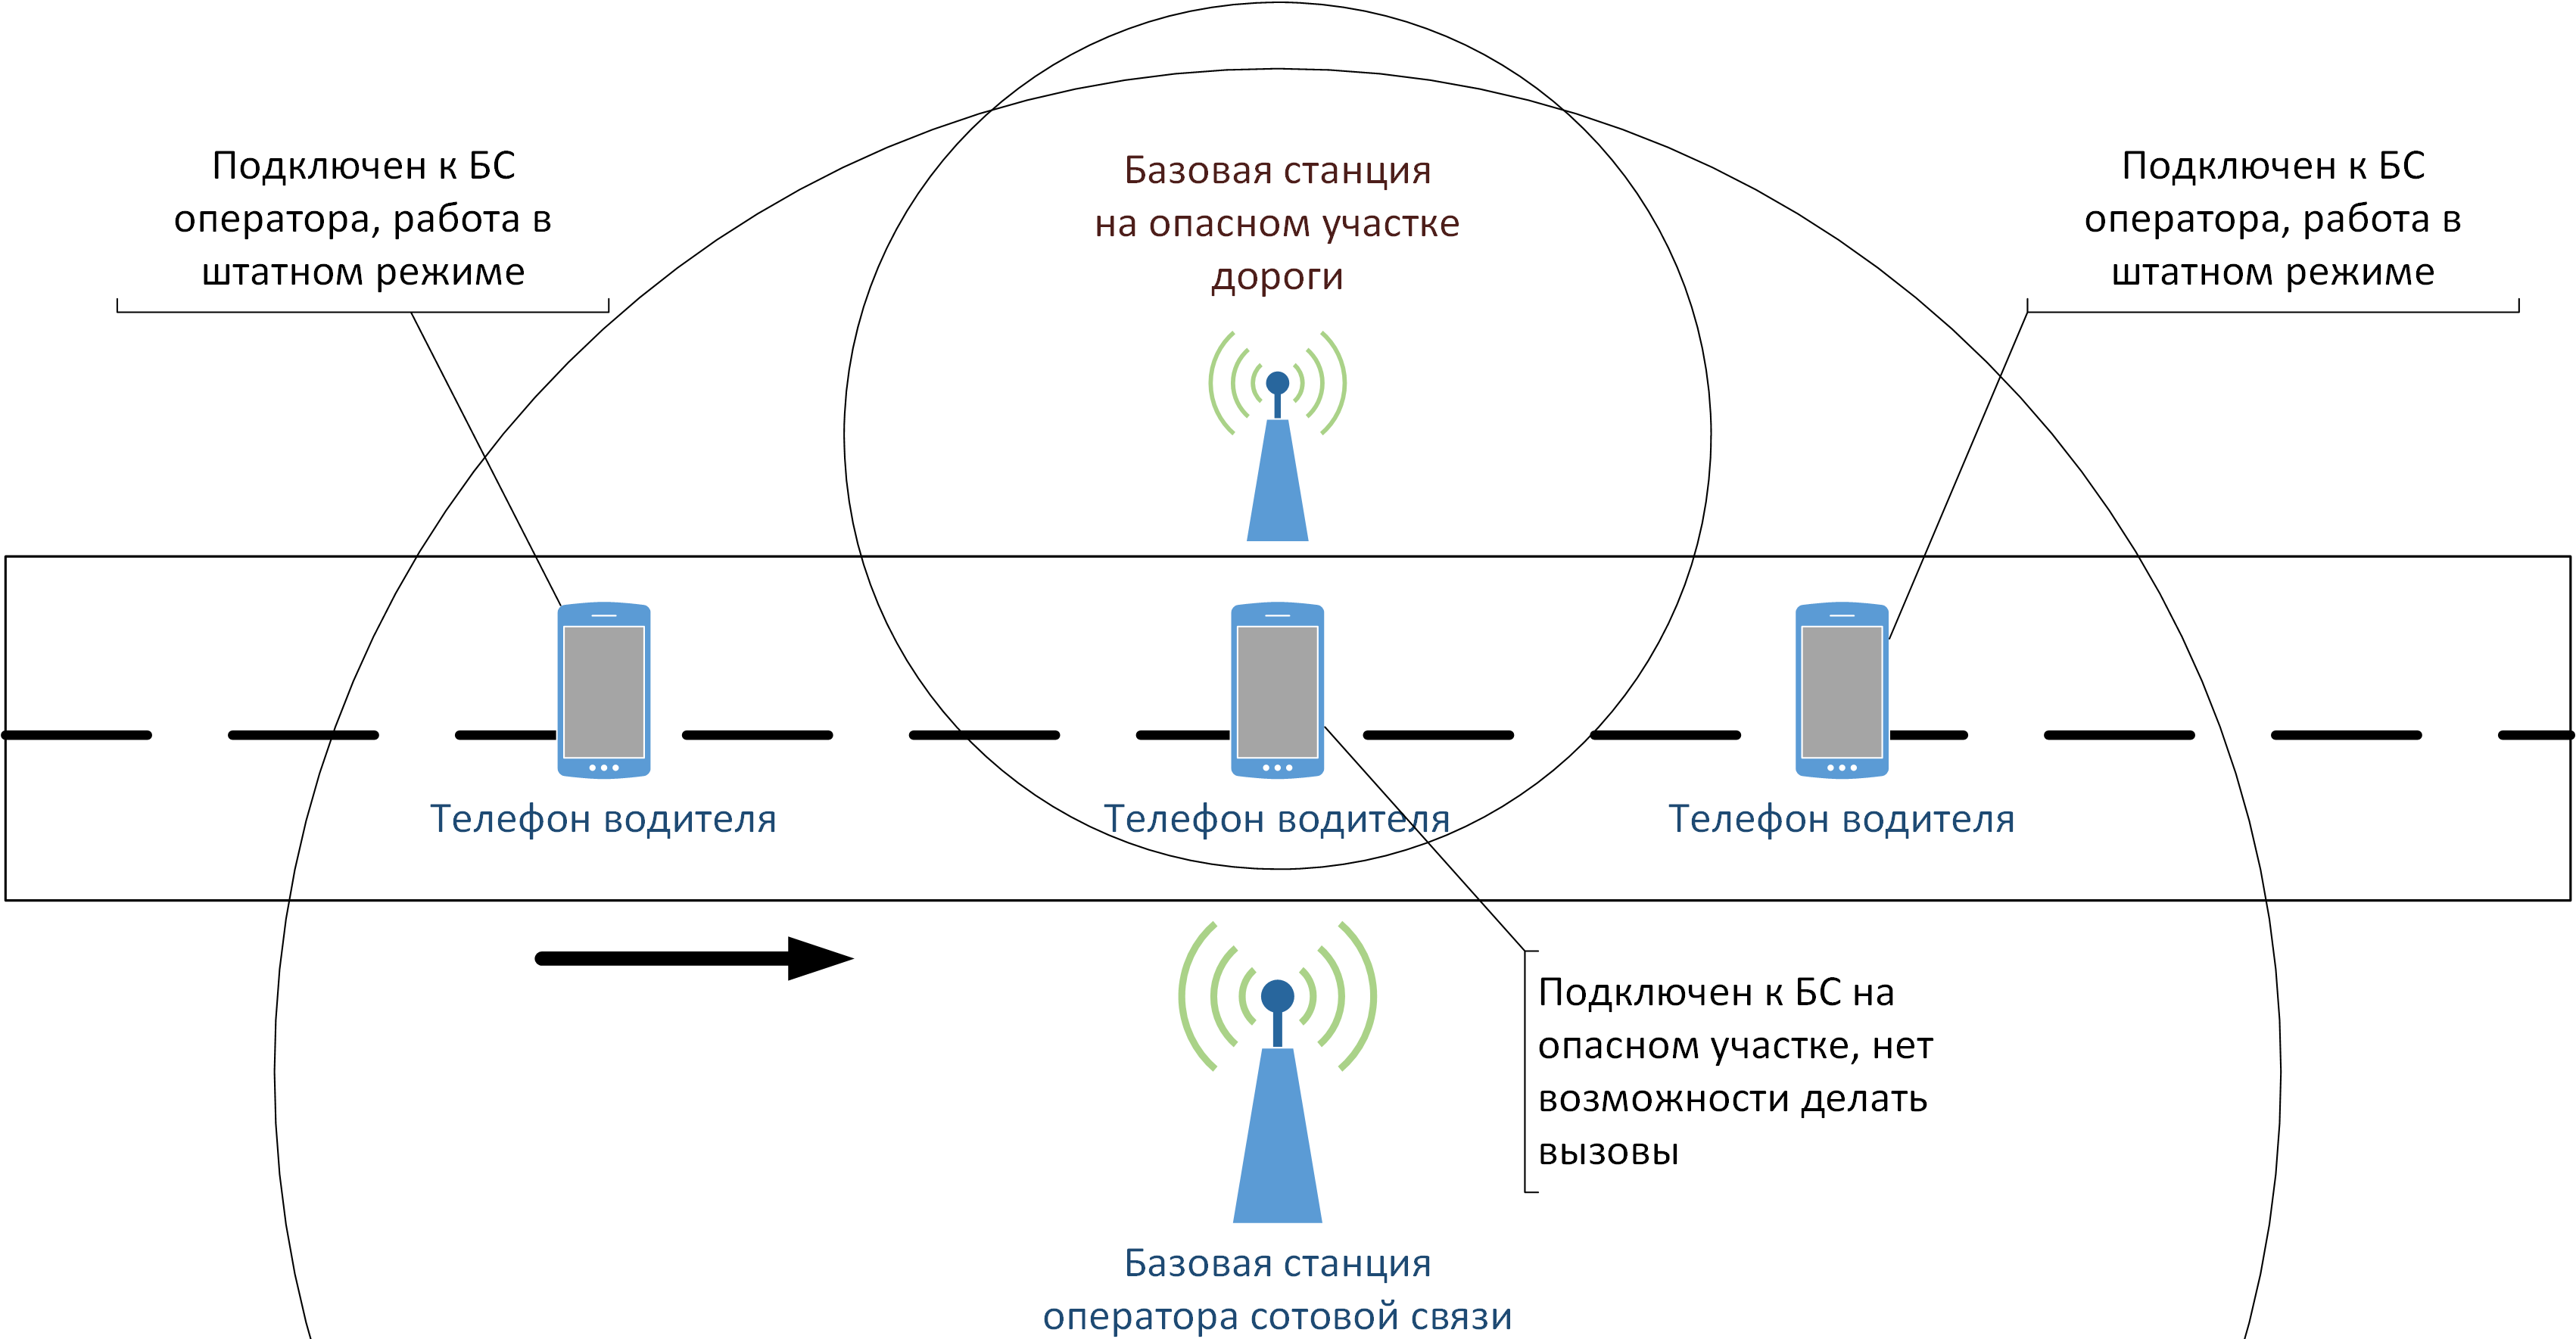
\includegraphics[width=0.7\textwidth]{BS_cut}
	\caption{Пояснение предложенного алгоритма}
	\label{fig:BS}
\end{figure}

После подключения сотового телефона к БС на опасном участке дороги разговор прерывается, если в момент переключения абонент разговаривал. Также прекращается действие таких услуг как SMS, мобильный интернет и т.д. Однако, после проезда опасного участка дороги, сотовый телефон вновь подключится к БС оператора связи, а это значит все возможности коммуникации будут восстановлены. Минусы предложенного метода заключаются в:
\begin{itemize}
	\item отсутствии в свободной продаже оборудования для запуска БС;
	\item необходимости лицензирования запускаемого оборудования;
	\item высокой совокупной стоимости запуска оборудования.
\end{itemize}

Однако, все вышеперечисленные минусы можно с легкостью обойти, законодательно обязав операторов сотовой связи устанавливать такие БС на опасных участках автодорог. Предполагается, что с введением таких мер водители будут осуществлять проезд опасного участка дороги и маневрирование на нем, управляя транспортным средством обеими руками и с более полной концентрацией внимания на изменения окружающей дорожной обстановки. Это будет способствовать снижению вероятности возникновения опасности для движения транспортных средств и пешеходов, а также создания аварийных ситуаций на дорогах.